\chapter{\red[Experimentelle ]Auswertung und Ergebnisse}
\label{chap.results}
\red[TODO:\\
PGFPlots einfügen\\
Daten aufbereiten\\
Ergebnisse vergleichen/auswerten\\
Versuchsdurchführungen beschreiben!? Skizzen?\\
]

Um die Funktionalität des \kps{s} bewerten und verschiedene Anwendungsfälle vergleichen zu können wird eine experimentelle Evaluation durchgeführt. Diese soll besonders dazu dienen, Fehlereinflüsse der aufeinander aufbauenden Transformationen zwischen der Lokalisation des Systems und der Darstellung der visuellen Zusatzinformationen zu quantifizieren.\\

Zunächst erfolgt eine Betrachtung der globalen Lokalisationsgenauigkeit, indem die zwei in \kapitel{chap.globloc} beschriebenen Modelle gegenübergestellt werden. Anschließend wird die Genauigkeit der lokalen Lokalisation bewertet, wobei die visuelle Odometrie und die mittels des EKF fusionierten Messdaten betrachtet werden. Abschließend wird eine gesonderte Auswertung des Projektionsvorgangs durchgeführt, welcher durch die Transformation zwischen Kamera und Projektor beschrieben wird.\\

Als Bewertungsreferenz \red[(Ground Truth)] der Lokalisation werden die in \abb{fig.armarker} gezeigten Markerfelder verwendet. Durch Erfassung in Kamerabildern können Orientierung und Ursprung der Felder bestimmt werden \red[näher erläuteren?]. Je Feld werden vier Marker aufgebracht um die Robustheit der Detektion zu erhöhen. Die jeweilige Positionierung der Felder ist abhängig von der jeweiligen Untersuchung und wird innerhalb der folgenden Abschnitte detaillierter beschrieben.\\

\begin{figure}[!ht]
	\begin{center}
	
	\subfigure[Markerfeld 1]{
		\begingroup\fboxsep=0pt\fboxrule=1pt
		\fbox{%
			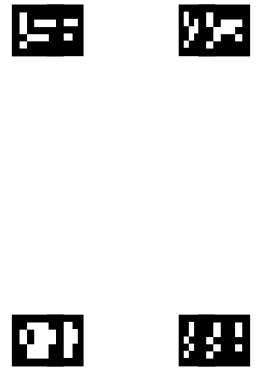
\includegraphics[scale=0.5]{ar_board_01}%
		}
		\endgroup
	}
	\hspace{5mm}
	\subfigure[Markerfeld 2]{
		\begingroup\fboxsep=0pt\fboxrule=1pt
		\fbox{%
			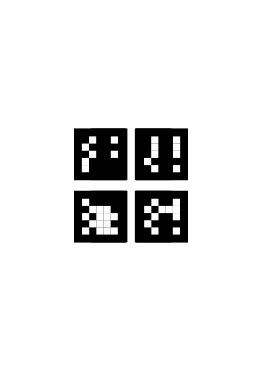
\includegraphics[scale=0.5]{ar_board_02}%	
		}
		\endgroup
	}
	\caption{AR Markerfelder}
	\label{fig.armarker}
	\end{center}
	%\vspace*{-8mm}
\end{figure}

Die betrachten Fehlerwerte $E$ werden dabei für alle Untersuchungen über die jeweiligen Einzeldifferenzen $r_i$ der $n$ Messungen als Quadratischer Mittelwert bestimmt:

\begin{equation}
E = \sqrt{\frac{1}{n}\sum_{i=1}^nr_i^2}
\end{equation}


\section{Globale Lokalisation}
Die globale Lokalisation bildet die Basis der Lagebestimmung des \kps{s}. Im folgenden werden das \red[Raycasting-] und das \red[Endpoint]-Modell verglichen und auf ihre Eignung als globales Lokalisationsverfahren geprüft. Neben der möglichst exakten Annäherung ist dabei auch eine approximative Bestimmung der Systempose von Bedeutung. Wird die Pose innerhalb eines Grenzbereiches angenähert, kann die verbleibende Abweichung durch anschließende Optimierungsschritte verringert werden. Im Falle einer fehlerhaften initialen Lokalisation kann jedoch trotz lokaler Optimierung nicht von einer Verringerung der Abweichung zur wahren Pose ausgegangen werden. Als zusätzliches Bewertungskriterium der globalen Lokalisation wird deshalb im Folgenden neben der Abweichung zur realen Pose auch die Erfolgsquote der Approximation erfasst. Als drittes Vergleichskriterium wird abschließend die für den Lokalisationsvorgang benötigte Rechenzeit ausgewertet.\\

%Dabei ist besonders eine approximative Bestimmung der Systempose von Bedeutung. Die Bestimmung einer möglichst exakten Annäherung der Pose ist zwar prinzipiell ebenso Ziel der globalen Lokalisation, kann jedoch bei korrekter initialer Approximation auch durch anschließende Optimierungsschritte erreicht werden. Im Falle einer fehlerhaften initialen Lokalisation kann trotz einer lokalen Optimierung nicht von einer Verringerung der Abweichung zur wahren Pose ausgegangen werden. Als zusätzliches Bewertungskriterium der globale Lokalisation wird deshalb im Folgenden neben der Abweichung zur realen Pose auch die Erfolgswahrscheinlichkeit der Approximation erfasst.\\

Um die wahre Pose des \kps{s} zu bestimmen wird das Markerfeld innerhalb der realen Umgebung auf einer glatten Fläche befestigt. Der Abgleich zwischen der daraus bestimmten Pose und der durch die Lokalisation ermittelten Pose ist dabei nur möglich, wenn die Pose des Markerfeldes auch in der Modellumgebung bekannt ist. Dies kann entweder durch Anbringung der Markerfelder vor der Kartierung oder durch Definition der Markerpose anhand eindeutiger Landmarken der Umgebung erreicht werden.\\

Die Bestimmung der Referenzpose kann nun durch Erfassung des Markerfeldes mit der Kamera des Systems erfolgen. Dazu wird das \kps{} in einer Pose fixiert und die Transformation zwischen dem Markerfeld und dem \kps{} bestimmt. Durch die vorhandene Verknüpfung zwischen der realen und der Modellumgebung ist die Transformation zwischen den Koordinaten der Karte und dem Markerfeld beschrieben\red[ Bild?]. Es lässt sich somit die Transformation zwischen \kps{} und Karte bestimmen zu:

\begin{equation}
\tmat{M}{K} = \tmat{M}{AR}\tmat{AR}{K}
\end{equation}

Auch die globale Lokalisation wird durchgeführt während sich das \kps{} in der fixierten Pose befindet. Für beide Modelle werden insgesamt $n=20.000$ Partikel zufällig in der Karte verteilt. Die jeweils ermittelte Pose mit der höchsten Wahrscheinlichkeit wird anschließen mit der Referenzposition verglichen. Die quadratischen Mittelwerte der Fehler bezüglich der translatorischen ($\Delta X$, $\Delta Y$, $\Delta Z$) und rotatorischen ($\Delta \Psi$, $\Delta \Theta$, $\Delta \Phi$) Freiheitsgrade des Systems sind in \abb{fig.glob_loc} in Abhängigkeit des verwendeten Modells aufgeführt.\\


\red[\abb{fig.error_glob_trans} zeigt den Vergleich der durch die beiden Modelle erzielten Fehlerwerte.\\]
\red[Versuchsparameter, Partikelzahl etc.]

\begin{center}
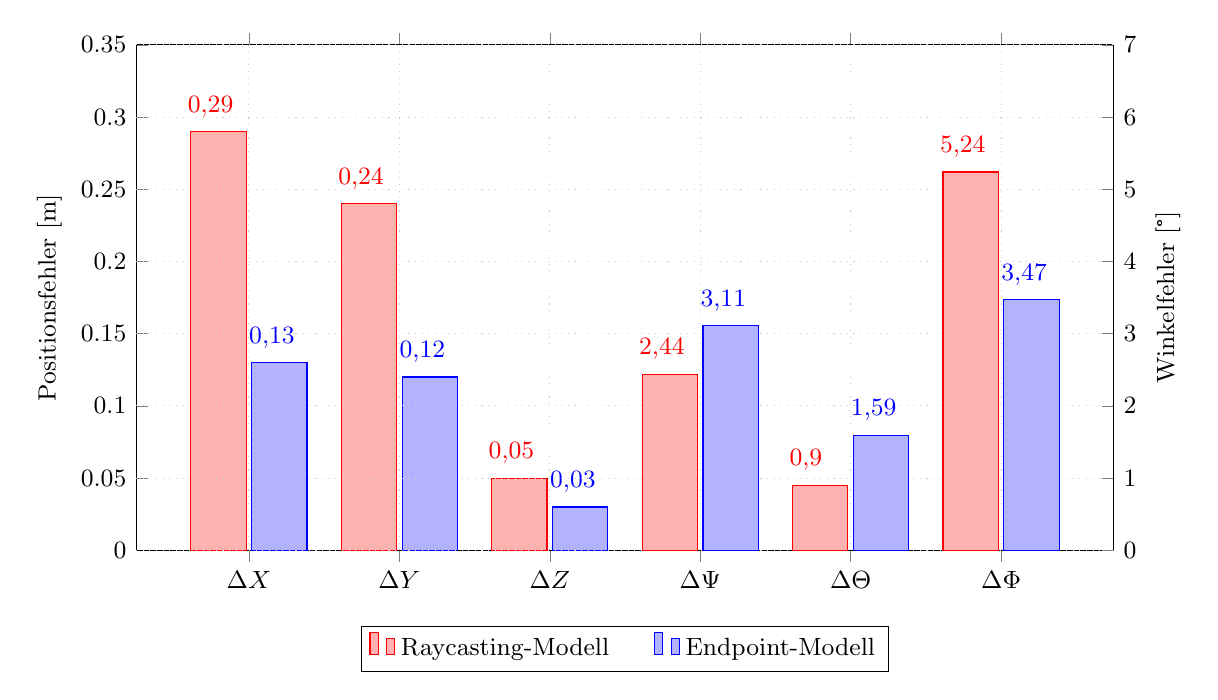
\begin{tikzpicture}
\tikzstyle{every node}=[font=\small]
\begin{axis}[
	ybar,
	ymax=0.35,
	ymin=0,
	bar width=20pt,
	scaled y ticks = false,
	y tick label style={/pgf/number format/fixed},
%	enlarge y limits={0.4,upper},
	enlarge x limits=0.15,
	legend style={at={(0.5,-0.15)},
	legend style={/tikz/every even column/.append style={column sep=0.5cm}},
	anchor=north,legend columns=-1},
	ylabel={Positionsfehler \lbrack m\rbrack},
%	symbolic x coords={\Delta,y,z},
	xtick={1,2,3,4,5,6},
	xticklabels={$\Delta X$, $\Delta Y$, $\Delta Z$, $\Delta \Psi$, $\Delta \Theta$, $\Delta \Phi$},
%	xtick=data,
	every node near coord/.style={/pgf/number format/fixed,/pgf/number format/use comma, anchor=west},
	nodes near coords,
	nodes near coords align={vertical},
	width=14cm,
	height=8cm,
	grid=major,
    	grid style={dotted,lightgray!80!white},
    	scaled y ticks = false,
]
\addplot[
	every node near coord/.append style={xshift=-0.9cm},
	nodes near coords=\raisebox{0.7cm}{\pgfmathprintnumber\pgfplotspointmeta},
	color=red,
	fill=red!30!white,
	bar shift=-11pt,
] coordinates {(1,0.29) (2,0.24) (3,0.05)};
\addplot[
	every node near coord/.append style={xshift=-0.12cm},
	nodes near coords=\raisebox{0.7cm}{\pgfmathprintnumber\pgfplotspointmeta},
	color=blue,
	fill=blue!30!white,
	bar shift=11pt,	
] coordinates {(1,0.13) (2,0.12) (3,0.03)};
\addplot[fill opacity=0.0,draw=none,] coordinates {(4,0) (5,0) (6,0)};	%dummy
\legend{Raycasting-Modell,Endpoint-Modell}
\end{axis}

\begin{axis}[
%	scale only axis,
	ybar,
	ymax=7,
	ymin=0,
	bar width=20pt,
%	enlarge y limits={0.4,upper},
	enlarge x limits=0.15,
	legend style={at={(0.5,-0.15)},
	anchor=north,legend columns=-1},
	axis y line*=right,
	axis x line=none,
	ylabel={Winkelfehler \lbrack °\rbrack},
%	symbolic x coords={\Delta,y,z},
	xtick={1,2,3,4,5,6},
	xticklabels={$\Delta X$, $\Delta Y$, $\Delta Z$, $\Delta \Psi$, $\Delta \Theta$, $\Delta \Phi$},
%	xtick=data,
%	bar shift=0pt,
	every node near coord/.style={/pgf/number format/fixed,/pgf/number format/use comma, anchor=west},
	nodes near coords,
	nodes near coords align={vertical},
	width=14cm,
	height=8cm,
	grid=major,
    	grid style={dotted,lightgray!80!white},
    	scaled y ticks = false,
]
\addplot[fill opacity=0.0,draw=none,] coordinates {(1,0) (2,0) (3,0)};	%dummy
\addplot[
	every node near coord/.append style={xshift=-0.9cm},
	nodes near coords=\raisebox{0.7cm}{\pgfmathprintnumber\pgfplotspointmeta},
	color=red,
	fill=red!30!white,
	bar shift=-11pt,	
] coordinates {(4,2.44) (5,0.90) (6,5.24)};
\addplot[
	every node near coord/.append style={xshift=-0.12cm},
	nodes near coords=\raisebox{0.7cm}{\pgfmathprintnumber\pgfplotspointmeta},
	color=blue,
	fill=blue!30!white,
	bar shift=11pt,	
] coordinates {(4,3.11) (5,1.59) (6,3.47)};
\end{axis}
\end{tikzpicture}
\end{center}

%\begin{center}
%\begin{tikzpicture}[trim axis left, trim axis right]
%\begin{axis}[
%	ybar,
%	ymax=0.4,
%	ymin=0,
%	bar width=30pt,
%	enlarge x limits=0.4,
%	legend style={at={(0.5,-0.15)},
%	anchor=north,legend columns=-1},
%	ylabel={Positionsfehler \lbrack m\rbrack},
%%	symbolic x coords={\Delta,y,z},
%	xticklabels={$\Delta X$, $\Delta Y$, $\Delta Z$},
%	xtick=data,
%	every node near coord/.style={/pgf/number format/fixed, anchor=west},
%	nodes near coords,
%	nodes near coords align={vertical},
%	width=14cm,
%	height=8cm,
%	grid=major,
%    	grid style={dotted,lightgray!80!white},
%    	scaled y ticks = false,
%]
%\addplot[
%	every node near coord/.append style={xshift=-1.1cm},
%	nodes near coords=\raisebox{0.7cm}{\pgfmathprintnumber\pgfplotspointmeta},
%	color=red,
%	fill=red!30!white
%] coordinates {(-1,0.3105647208) (0,0.3388888731) (1,0.0473358078)};
%\addplot[
%	every node near coord/.append style={xshift=0.0cm},
%	nodes near coords=\raisebox{0.7cm}{\pgfmathprintnumber\pgfplotspointmeta},
%	color=blue,
%	fill=blue!30!white
%] coordinates {(-1,0.1315834135) (0,0.1248760865) (1,0.0209899568)};
%\legend{Raycasting,Endpoint}
%\end{axis}
%\label{fig.error_glob_trans}
%\end{tikzpicture}
%\end{center}
%
%\red[Winkelfehler Vergleich:\\]
%
%\begin{center}
%\begin{tikzpicture}[trim axis left, trim axis right]
%\begin{axis}[
%	ybar,
%	ymax=10,
%	ymin=0,
%	bar width=30pt,
%%	enlarge y limits={0.4,upper},
%	enlarge x limits=0.4,
%	legend style={at={(0.5,-0.15)},
%	anchor=north,legend columns=-1},
%	ylabel={Winkelfehler \lbrack °\rbrack},
%%	symbolic x coords={\Delta,y,z},
%	xticklabels={$\Delta \Psi$, $\Delta \Theta$, $\Delta \Phi$},
%	xtick=data,
%	every node near coord/.style={/pgf/number format/fixed, anchor=west},
%	nodes near coords,
%	nodes near coords align={vertical},
%	width=14cm,
%	height=8cm,
%	grid=major,
%    	grid style={dotted,lightgray!80!white},
%    	scaled y ticks = false,
%]
%\addplot[
%	every node near coord/.append style={xshift=-1.1cm},
%	nodes near coords=\raisebox{0.7cm}{\pgfmathprintnumber\pgfplotspointmeta},
%	color=red,
%	fill=red!30!white
%] coordinates {(-1,2.4445637073) (0,0.9069805767) (1,8.4545773848)};
%\addplot[
%	every node near coord/.append style={xshift=0.0cm},
%	nodes near coords=\raisebox{0.7cm}{\pgfmathprintnumber\pgfplotspointmeta},
%	color=blue,
%	fill=blue!30!white
%] coordinates {(-1,3.1694824628) (0,1.6633422885) (1,4.2398218425)};
%\legend{Raycasting,Endpoint}
%\end{axis}
%\label{fig.error_glob_rot}
%\end{tikzpicture}
%\end{center}


%\begin{figure}[!ht]
%	\begin{center}
%	\subfigure[1. Formparameter (Fokus-Modell)]{
%		\begin{tikzpicture}[scale=0.6, baseline]
%            \begin{axis}[ybar]
%                \addplot+ coordinates {
%                    (1,2)
%                };
%            \end{axis}
%        \end{tikzpicture}
%	}
%	\hspace{2mm}
%	\subfigure[1. Formparameter (Post-Fokus-Modell)]{
%		\begin{tikzpicture}[scale=0.6, baseline]
%            \begin{axis}[ybar]
%                \addplot+ coordinates {
%                    (1,2)
%                };
%            \end{axis}
%        \end{tikzpicture}
%	}\\
%	\caption{Variation der ersten beiden Formparameter um $\pm 3 \sqrt{\lambda_i}$}
%	\label{fig.reference_building_shape_visualization}
%	\end{center}
%	\vspace*{-8mm}
%\end{figure}

Aufgrund der Programmstruktur ist die Vorgabe eines Bereiches zur Verteilung der Partikel bezüglich der \red[z-Koordinate] der Karte erforderlich. Da das handgeführte \kps{} zu Beginn der Anwendung leicht in einer definierten Höhe bewegt werden kann, wurde dieser Grenzbereich mit einer Toleranz von $\pm$ \SI{0,1}{\meter} zur tatsächlichen Pose definiert. Die Fehlerwerte bezüglich dieses Freiheitsgrades können aufgrund dieser Vorgabe nicht über der gewählten Toleranz liegen.\\

\red[Ergebnisse beschreiben und interpretieren\\]

\red[Definition, welche als erfolgreich gelten müsste eigentlich vorher schon kommen um daraus die Fehlerwerte zu berechnen!\\]

Um die erfolgreiche Approximation der Pose zu bewerten wird wie in \abb{fig.loclimits} dargestellt ein Grenzraum um die wahre Position des \kps{s} definiert. Für die maximal zulässigen Winkelfehler werden ebenfalls Grenzbereiche festgelegt. Die Grenzwerte sind in \tab{thresh_glob} aufgeführt und orientieren sich an den Fehlerwerten, aus welchen durch das von Forster \textit{et al.} \cite{Forster2013} vorgestellte Verfahren eine Optimierung der Pose erreicht werden konnte.\\
%\red[Festgelegt nach \cite{Forster2013}\\]

\begin{figure}[!ht]
	\begin{center}
		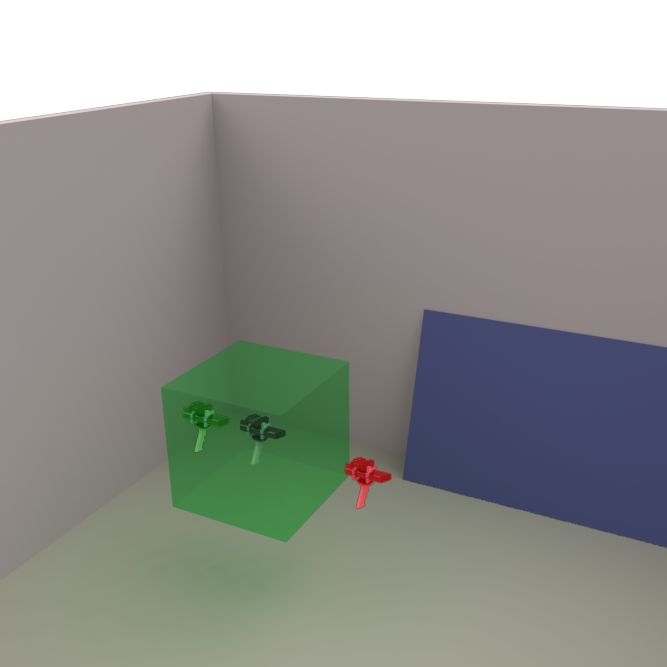
\includegraphics[scale=1.0]{glob_loc_thresh_02}
		\caption{Grenzbereich der Lokalisation}
		\label{fig.loclimits}
	\end{center}
	%\vspace*{-8mm}
\end{figure}

\begin{table}[ht]
	\centering
	\caption{Grenzwerte zur Bestimmung der erfolgreichen Approximation}
	\label{tab.thresh_glob}
	\vspace*{-3mm}
	\begin{tabular}[ht]{|l|r|}\hline
		\rowcolor{Snow2}
		Dimension		& Grenzwert 					\\ \hline
		X				& \SI{0,35}{\meter}			\\ \hline		
		Y				& \SI{0,35}{\meter}			\\ \hline
		Z				& \SI{0,35}{\meter}			\\ \hline
		Yaw				& \SI{7}{°}					\\ \hline
		Pitch			& \SI{7}{°}					\\ \hline
		Roll 			& \SI{7}{°}					\\ \hline
	\end{tabular} 
	\vspace*{-3mm}
\end{table}

Die Erfolgsquote der Annäherung der wahren Systempose berechnet sich aus dem Quotienten der fehlgeschlagenen und insgesamt durchgeführten Lokalisationen. Als fehlgeschlagen werden dabei alle Lokalisationen betrachtet, bei welchen einer der definierten Grenzwerte überschritten wurde. Die Ergebnisse sind zusammen mit der durchschnittlich für die globale Lokalisation benötigten Rechenzeit $\bar{t}$ in \tab{approx_time} aufgeführt.

\begin{table}[ht]
	\centering
	\caption{Ermittelte Erfolgsquote und benötigte Rechenzeit}
	\label{tab.approx_time}
	\vspace*{-3mm}
	\begin{tabular}[ht]{|l|r|r|}\hline
		\rowcolor{Snow2}
		Modell			& Erfolgsquote [$\%$]	&	Rechenzeit $\bar{t}$	 [s]	\\ \hline
		Raycasting		& 56,25					&	\SI{532,89}{}			\\ \hline		
		Endpoint			& 75					&	\SI{55,66}{}			\\ \hline
	\end{tabular} 
	\vspace*{-3mm}
\end{table}

\red[Erfolgsquote interpretieren\\]

Wie aus \tab{approx_time} darüber hinaus ersichtlich wird, beträgt die benötigte Rechenzeit des \red[Raycasting]-Modells fast das \SI{10}{}-fache der vom \red[Endpoint]-Model benötigten Zeit. 
\red[Zeit der Lokalisation auswerten\\]

\red[Fazit daraus ableiten, welches besser geeignet ist? oder erst im Fazit/Zusammenfassung?\\]


\red[Quadratischer Mittelwert QMW statt Root Mean Square RMS überall aktualisieren\\]


\red[Relokalisation bei globaler Lokalisation beschreiben. Besser später als Ergänzung um die lokale Lokalisation zu korrigieren!\\]

\section{Lokale Lokalisation}%Tracking/Kontinuierliche Lokalisation}
Die Genauigkeit der lokalen Lokalisation wird gesondert von der durch die globale Lokalisation bestimmten Pose betrachtet. Dazu wird ebenfalls das für die Untersuchung der globalen Lokalisation verwendete Markerfeld genutzt. Die wahre Pose des Systems kann so wie zuvor bestimmt und als Initialisierung der Lokalisation verwendet werden.\\

Die Bewertung der kontinuierlichen Lokalisation erfolgt für translatorische und rotatorische Veränderungen der Systempose. Alle Messungen werden dabei separat durchgeführt um eine Beeinflussung der Bewegungen untereinander zu vermeiden.\\

\subsection{Translatorische Bewegung}
Die translatorischen Bewegungen werden parallel (x-Achse der Kamera, y-Achse des Systems) und orthogonal (z-Achse der Kamera, x-Achse des Systems) zu der Betrachtungsebene durchgeführt. Die parallele Bewegung entlang der zweiten zur Ebene parallelen Achse (y-Achse der Kamera, z-Achse des Systems) wird nicht gesondert betrachtet, da diese äquivalent zu der Bewegung entlang der ersten ist. \abb{fig.transmove} verdeutlicht dies und zeigt die Durchführung der Untersuchungen anhand eines beispielhaften Versuchsaufbaus.\\

\begin{figure}[!ht]
	\begin{center}
		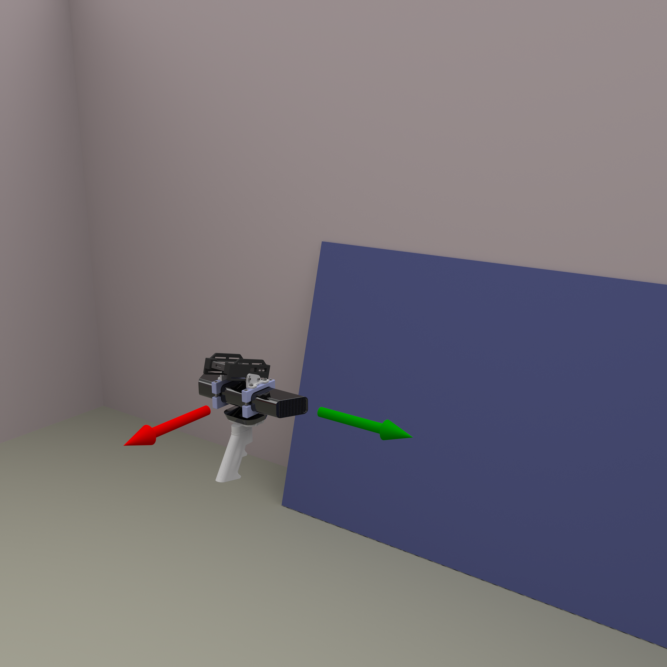
\includegraphics[scale=1.0]{loc_loc_lin}
		\caption{Translatorische Bewegung}
		\label{fig.transmove}
	\end{center}
	%\vspace*{-8mm}
\end{figure}

Die quadratischen Mittelwerte der Lokalisationsfehler bei translatorischen Bewegungen parallel und orthogonal zur Betrachtungsebene sind in \abb{fig.loc_loc_trans} dargestellt.

%---------------------------------- Translatorische Bewegung kombiniert in einem Diagramm für alle Freiheitsgrade--------------------------
\begin{center}
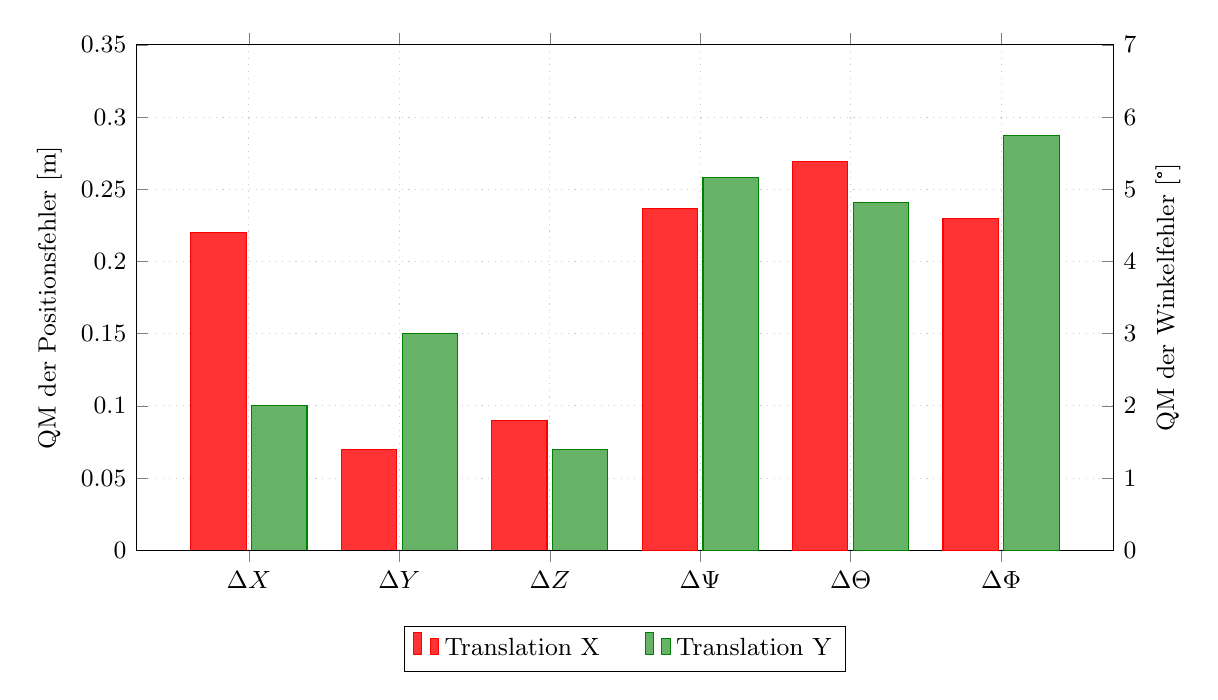
\begin{tikzpicture}
\begin{axis}[
	ybar,
	ymax=0.35,
	ymin=0,
	bar width=20pt,
	scaled y ticks = false,
	y tick label style={/pgf/number format/fixed},
%	enlarge y limits={0.4,upper},
	enlarge x limits=0.15,
	legend style={at={(0.5,-0.15)},
	legend style={/tikz/every even column/.append style={column sep=0.5cm}},
	anchor=north,legend columns=-1},
	ylabel={QM der Positionsfehler \lbrack m\rbrack},
%	symbolic x coords={\Delta,y,z},
	xtick={1,2,3,4,5,6},
	xticklabels={$\Delta X$, $\Delta Y$, $\Delta Z$, $\Delta \Psi$, $\Delta \Theta$, $\Delta \Phi$},
%	xtick=data,
%	every node near coord/.style={/pgf/number format/fixed,/pgf/number format/use comma, anchor=west},
%	nodes near coords,
%	nodes near coords align={vertical},
	width=14cm,
	height=8cm,
	grid=major,
    	grid style={dotted,lightgray!80!white},
    	scaled y ticks = false,
]
\addplot[
%	every node near coord/.append style={xshift=-0.9cm},
%	nodes near coords=\raisebox{0.7cm}{\pgfmathprintnumber\pgfplotspointmeta},
	color=Red,
	fill=Red!80!white,
	bar shift=-11pt,
] coordinates {(1,0.22) (2,0.07) (3,0.09)};
\addplot[
%	every node near coord/.append style={xshift=-0.12cm},
%	nodes near coords=\raisebox{0.7cm}{\pgfmathprintnumber\pgfplotspointmeta},
	color=Green,
	fill=Green!60!white,
	bar shift=11pt,	
] coordinates {(1,0.10) (2,0.15) (3,0.07)};
\addplot[fill opacity=0.0,draw=none,] coordinates {(4,0) (5,0) (6,0)};	%dummy
\legend{Translation X,Translation Y}
\end{axis}

\begin{axis}[
%	scale only axis,
	ybar,
	ymax=7,
	ymin=0,
	bar width=20pt,
%	enlarge y limits={0.4,upper},
	enlarge x limits=0.15,
	legend style={at={(0.5,-0.15)},
	anchor=north,legend columns=-1},
	axis y line*=right,
	ylabel={QM der Winkelfehler \lbrack °\rbrack},
%	symbolic x coords={\Delta,y,z},
	xtick={1,2,3,4,5,6},
	xticklabels={},
%	xtick=data,
%	bar shift=0pt,
%	every node near coord/.style={/pgf/number format/fixed,/pgf/number format/use comma, anchor=west},
%	nodes near coords,
%	nodes near coords align={vertical},
	width=14cm,
	height=8cm,
    	scaled y ticks = false,
]
\addplot[fill opacity=0.0,draw=none,] coordinates {(1,0) (2,0) (3,0)};	%dummy
\addplot[
%	every node near coord/.append style={xshift=-0.9cm},
%	nodes near coords=\raisebox{0.7cm}{\pgfmathprintnumber\pgfplotspointmeta},
	color=Red,
	fill=Red!80!white,
	bar shift=-11pt,	
] coordinates {(4,4.73) (5,5.39) (6,4.59)};
\addplot[
%	every node near coord/.append style={xshift=-0.12cm},
%	nodes near coords=\raisebox{0.7cm}{\pgfmathprintnumber\pgfplotspointmeta},
	color=Green,
	fill=Green!60!white,
	bar shift=11pt,	
] coordinates {(4,5.16) (5,4.82) (6,5.75)};
\end{axis}
\end{tikzpicture}
\end{center}

%----------------------------------------------------------------------------------------------------------
%------------------------------------------  Anfang  ------------------------------------------------------
%------------------------ Vergleich mit xyz rpy in getrennten Diagrammen ----------------------------------
%----------------------------------------------------------------------------------------------------------
%----------------------------------------------------------------------------------------------------------
%\subsection{Translatorische Bewegung}
%\begin{center}
%\begin{tikzpicture}[trim axis left, trim axis right]
%\begin{axis}[
%	ybar,
%	ymax=0.25,
%	ymin=0,
%	bar width=30pt,
%	enlarge x limits=0.4,
%	legend style={at={(0.5,-0.15)},
%	anchor=north,legend columns=-1},
%	ylabel={Positionsfehler \lbrack m\rbrack},
%%	symbolic x coords={\Delta,y,z},
%	xticklabels={$\Delta X$, $\Delta Y$, $\Delta Z$},
%	xtick=data,
%	every node near coord/.style={/pgf/number format/fixed, anchor=west},
%	nodes near coords,
%	nodes near coords align={vertical},
%	width=14cm,
%	height=8cm,
%	grid=major,
%    	grid style={dotted,lightgray!80!white},
%    	scaled y ticks = false,
%	y tick label style={/pgf/number format/fixed},
%]
%\addplot[
%	every node near coord/.append style={xshift=-1.1cm},
%	nodes near coords=\raisebox{0.7cm}{\pgfmathprintnumber\pgfplotspointmeta},
%	color=red,
%	fill=red!30!white
%] coordinates {(-1,0.0942737252) (0,0.0744944439) (1,0.2154737652)};
%\addplot[
%	every node near coord/.append style={xshift=0.0cm},
%	nodes near coords=\raisebox{0.7cm}{\pgfmathprintnumber\pgfplotspointmeta},
%	color=blue,
%	fill=blue!30!white
%] coordinates {(-1,0.0141228693) (0,0.0728502984) (1,0.0578491359)};
%\legend{Translatorsich X,Translatorisch Z}
%\end{axis}
%\label{fig.error_glob_trans}
%\end{tikzpicture}
%\end{center}
%
%\begin{center}
%\begin{tikzpicture}[trim axis left, trim axis right]
%\begin{axis}[
%	ybar,
%	ymax=8,
%	ymin=0,
%	bar width=30pt,
%%	enlarge y limits={0.4,upper},
%	enlarge x limits=0.4,
%	legend style={at={(0.5,-0.15)},
%	anchor=north,legend columns=-1},
%	ylabel={Winkelfehler \lbrack °\rbrack},
%%	symbolic x coords={\Delta,y,z},
%	xticklabels={$\Delta \Psi$, $\Delta \Theta$, $\Delta \Phi$},
%	xtick=data,
%	every node near coord/.style={/pgf/number format/fixed, anchor=west},
%	nodes near coords,
%	nodes near coords align={vertical},
%	width=14cm,
%	height=8cm,
%	grid=major,
%    	grid style={dotted,lightgray!80!white},
%    	scaled y ticks = false,
%	y tick label style={/pgf/number format/fixed},    	
%]
%\addplot[
%	every node near coord/.append style={xshift=-1.1cm},
%	nodes near coords=\raisebox{0.7cm}{\pgfmathprintnumber\pgfplotspointmeta},
%	color=red,
%	fill=red!30!white
%] coordinates {(-1,5.3910094725) (0,0.5944624236) (1,4.7266768476)};
%\addplot[
%	every node near coord/.append style={xshift=0.0cm},
%	nodes near coords=\raisebox{0.7cm}{\pgfmathprintnumber\pgfplotspointmeta},
%	color=blue,
%	fill=blue!30!white
%] coordinates {(-1,3.3292065305) (0,1.4935343647) (1,6.1138224963)};
%\legend{Translatorisch X,Translatorisch Z}
%\end{axis}
%\label{fig.error_loc_trans}
%\end{tikzpicture}
%\end{center}
%----------------------------------------------------------------------------------------------------------
%-------------------------------------------  Ende  -------------------------------------------------------
%------------------------ Vergleich mit xyz rpy in getrennten Diagrammen ----------------------------------
%----------------------------------------------------------------------------------------------------------
%----------------------------------------------------------------------------------------------------------

%----------------------------------------------------------------------------------------------------------
%------------------------------------------  Anfang  ------------------------------------------------------
%---------------- Vergleich mit xyz rpy in einem Diagramm, getrennt nach x und z --------------------------
%----------------------------------------------------------------------------------------------------------
%----------------------------------------------------------------------------------------------------------
%\subsection{Translation X}
%\begin{tikzpicture}
%\begin{axis}[
%	ybar,
%	ymax=0.3,
%	ymin=0,
%	bar width=30pt,
%	scaled y ticks = false,
%	y tick label style={/pgf/number format/fixed},
%% 	enlarge y limits={0.4,upper},
%	enlarge x limits=0.2,
%	legend style={at={(0.5,-0.15)},
%	anchor=north,legend columns=-1},
%	ylabel={Positionsfehler \lbrack m\rbrack},
%% 	symbolic x coords={\Delta,y,z},
%	xtick={1,2,3,4,5,6},
%	xticklabels={$\Delta X$, $\Delta Y$, $\Delta Z$, $\Delta \Psi$, $\Delta \Theta$, $\Delta \Phi$},
%% 	xtick=data,
%	bar shift=0pt,
%	every node near coord/.style={/pgf/number format/fixed, anchor=west},
%	nodes near coords,
%	nodes near coords align={vertical},
%	width=14cm,
%	height=8cm,
%	grid=major,
%	grid style={dotted,lightgray!80!white},
%	scaled y ticks = false,
%]
%\addplot[
%	every node near coord/.append style={xshift=-0.55cm},
%	nodes near coords=\raisebox{0.7cm}{\pgfmathprintnumber\pgfplotspointmeta},
%	color=red,
%	fill=red!30!white
%] coordinates {(1,0.0942737252) (2,0.0744944439) (3,0.2154737652)};
%\addplot[fill opacity=0.0,draw=none,] coordinates {(4,0) (5,0) (6,0)}; %dummy
%%\legend{Raycasting,Endpoint}
%\end{axis}
%
%\begin{axis}[
%% 	scale only axis,
%	ybar,
%	ymax=6,
%	ymin=0,
%	bar width=30pt,
%% 	enlarge y limits={0.4,upper},
%	enlarge x limits=0.2,
%	legend style={at={(0.5,-0.15)},
%	anchor=north,legend columns=-1},
%	axis y line*=right,
%	axis x line=none,
%	ylabel={Winkelfehler \lbrack °\rbrack},
%% 	symbolic x coords={\Delta,y,z},
%	xtick={1,2,3,4,5,6},
%	xticklabels={$\Delta X$, $\Delta Y$, $\Delta Z$, $\Delta \Psi$, $\Delta \Theta$, $\Delta \Phi$},
%% 	xtick=data,
%	bar shift=0pt,
%	every node near coord/.style={/pgf/number format/fixed, anchor=west},
%	nodes near coords,
%	nodes near coords align={vertical},
%	width=14cm,
%	height=8cm,
%	grid=major,
%	grid style={dotted,lightgray!80!white},
%	scaled y ticks = false,
%]
%\addplot[fill opacity=0.0,draw=none,] coordinates {(1,0) (2,0) (3,0)}; %dummy
%\addplot[
%	every node near coord/.append style={xshift=-0.55cm},
%	nodes near coords=\raisebox{0.7cm}{\pgfmathprintnumber\pgfplotspointmeta},
%	color=blue,
%	fill=blue!30!white,
%	% fill opacity=0.5,
%	% draw=none,
%] coordinates {(4,5.3910094725) (5,0.5944624236) (6,4.7266768476)};
%\end{axis}
%\label{fig.error_glob_trans_x}
%\end{tikzpicture}
%
%\subsection{Translation Z}
%\begin{tikzpicture}
%\begin{axis}[
%	ybar,
%	ymax=0.2,
%	ymin=0,
%	bar width=30pt,
%	scaled y ticks = false,
%	y tick label style={/pgf/number format/fixed},
%%	enlarge y limits={0.4,upper},
%	enlarge x limits=0.2,
%	legend style={at={(0.5,-0.15)},
%	anchor=north,legend columns=-1},
%	ylabel={Positionsfehler \lbrack m\rbrack},
%%	symbolic x coords={\Delta,y,z},
%	xtick={1,2,3,4,5,6},
%	xticklabels={$\Delta X$, $\Delta Y$, $\Delta Z$, $\Delta \Psi$, $\Delta \Theta$, $\Delta \Phi$},
%%	xtick=data,
%	bar shift=0pt,
%	every node near coord/.style={/pgf/number format/fixed, anchor=west},
%	nodes near coords,
%	nodes near coords align={vertical},
%	width=14cm,
%	height=8cm,
%	grid=major,
%    	grid style={dotted,lightgray!80!white},
%    	scaled y ticks = false,
%]
%\addplot[
%	every node near coord/.append style={xshift=-0.55cm},
%	nodes near coords=\raisebox{0.7cm}{\pgfmathprintnumber\pgfplotspointmeta},
%	color=red,
%	fill=red!30!white
%] coordinates {(1,0.0141228693) (2,0.0728502984) (3,0.0578491359)};
%\addplot[fill opacity=0.0,draw=none,] coordinates {(4,0) (5,0) (6,0)};	%dummy
%%\legend{Raycasting,Endpoint}
%\end{axis}
%
%\begin{axis}[
%%	scale only axis,
%	ybar,
%	ymax=8,
%	ymin=0,
%	bar width=30pt,
%%	enlarge y limits={0.4,upper},
%	enlarge x limits=0.2,
%	legend style={at={(0.5,-0.15)},
%	anchor=north,legend columns=-1},
%	axis y line*=right,
%	axis x line=none,
%	ylabel={Winkelfehler \lbrack °\rbrack},
%%	symbolic x coords={\Delta,y,z},
%	xtick={1,2,3,4,5,6},
%	xticklabels={$\Delta X$, $\Delta Y$, $\Delta Z$, $\Delta \Psi$, $\Delta \Theta$, $\Delta \Phi$},
%%	xtick=data,
%	bar shift=0pt,
%	every node near coord/.style={/pgf/number format/fixed, anchor=west},
%	nodes near coords,
%	nodes near coords align={vertical},
%	width=14cm,
%	height=8cm,
%	grid=major,
%    	grid style={dotted,lightgray!80!white},
%    	scaled y ticks = false,
%]
%\addplot[fill opacity=0.0,draw=none,] coordinates {(1,0) (2,0) (3,0)};	%dummy
%\addplot[
%	every node near coord/.append style={xshift=-0.55cm},
%	nodes near coords=\raisebox{0.7cm}{\pgfmathprintnumber\pgfplotspointmeta},
%	color=blue,
%	fill=blue!30!white,
%%	fill opacity=0.5,
%%	draw=none,
%] coordinates {(4,3.3292065305) (5,1.4935343647) (6,6.1138224963)};
%%\addplot[
%%	every node near coord/.append style={xshift=-1.1cm},
%%	nodes near coords=\raisebox{0.7cm}{\pgfmathprintnumber\pgfplotspointmeta},
%%	color=red,
%%	fill=red!30!white
%%] coordinates {(-2,0) (-1,0) (0,0) (1,2.4445637073) (2,0.9069805767) (3,8.4545773848)};
%\end{axis}
%\label{fig.error_glob_trans_x}
%\end{tikzpicture}
%----------------------------------------------------------------------------------------------------------
%-------------------------------------------  Ende  -------------------------------------------------------
%--------------------------- Vergleich mit xyz rpy in einem Diagramm --------------------------------------
%----------------------------------------------------------------------------------------------------------
%----------------------------------------------------------------------------------------------------------

\red[Ergebnisse interpretieren\\]
%\red[TransX und TransZ innerhalb vergleichen und Diagramme aufteilen nach translatorischem Fehler und rotatorischem Fehler?\\Oder direkt alles in einem -> 2x6 Balken!?]

\subsection{Rotatorische Bewegung}
\red[Vergleich zwischen Fovis und Fovis+IMU direkt zusammen in Diagramm aufführen? Erstmal nur Fovis würde dazu dienen, die Bewegungen untereinander zu vergleichen, aber was für Erkenntnisse erhält man daraus? Nick schlechter als Roll ; Nick durch IMU verbessert? -> Kompass sinnvoll! Dann evtl. aber ruhig auch Gierwinkelbewegung aufführen!\\]
Die Lokalisation während der Rotationsbewegungen wird zunächst allein auf Basis der visuellen Odometrie durchgeführt. Um die Fusion der Sensordaten mit den Daten der inertialen Messeinheit zu bewerten erfolgt anschließend ein Vergleich mit der Lokalisation auf Basis des Erweiterten Kalman Filters.\\
\red[Analog zur Auswertung der translatorischen Bewegungen werden lediglich die resultierenden Fehler aus den Rotationen um die Roll- und Nickachse ausgewertet. Die Rotation des Systems um die Gier-Achse unterscheidet sich für den Algorithmus der visuellen Odometrie nicht von der Rotation um die Nickachse, weshalb keine gesonderte Betrachtung durchgeführt wird.] Die Versuchsdurchführung der Bewegungen zur Bewertung der rotatorischen Fehlereinflüsse zeigt \abb{fig.rotmove}\\
\red[ypr alle aufführen oder nur roll und pitch, da yaw äquivalent zu pitch ist!? s.o.\\]

\begin{figure}[!ht]
	\begin{center}
		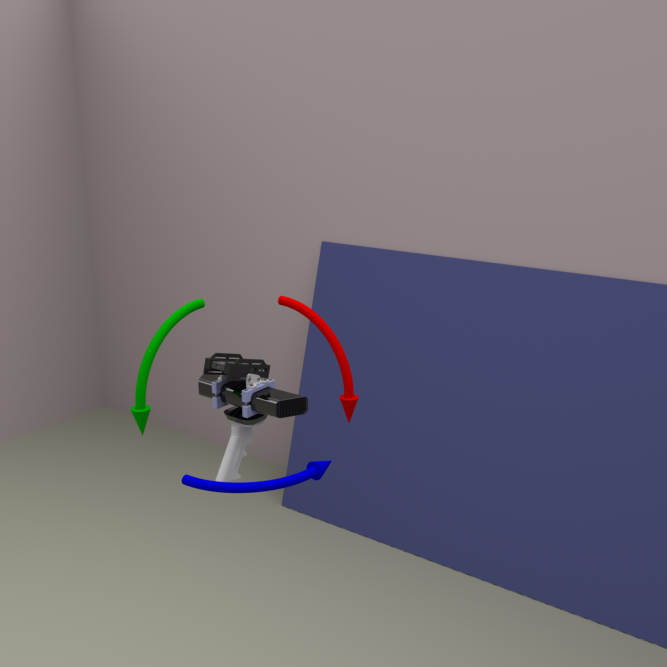
\includegraphics[scale=1.0]{loc_loc_rot}
		\caption{Rotatorische Bewegung}
		\label{fig.rotmove}
	\end{center}
	%\vspace*{-8mm}
\end{figure}

\red[Bilder des Aufbaus als subfigures!]

\subsubsection{Visuelle Odometrie}
Die aus den rotatorischen Bewegungen resultierenden Fehler in der ermittelten Systempose zeigt \abb{fig.loc_loc_rot_fovis_roll} für die Rotation um die Roll- und \abb{fig.loc_loc_rot_fovis_pitch} für die Rotation um die Nickachse.

\begin{center}
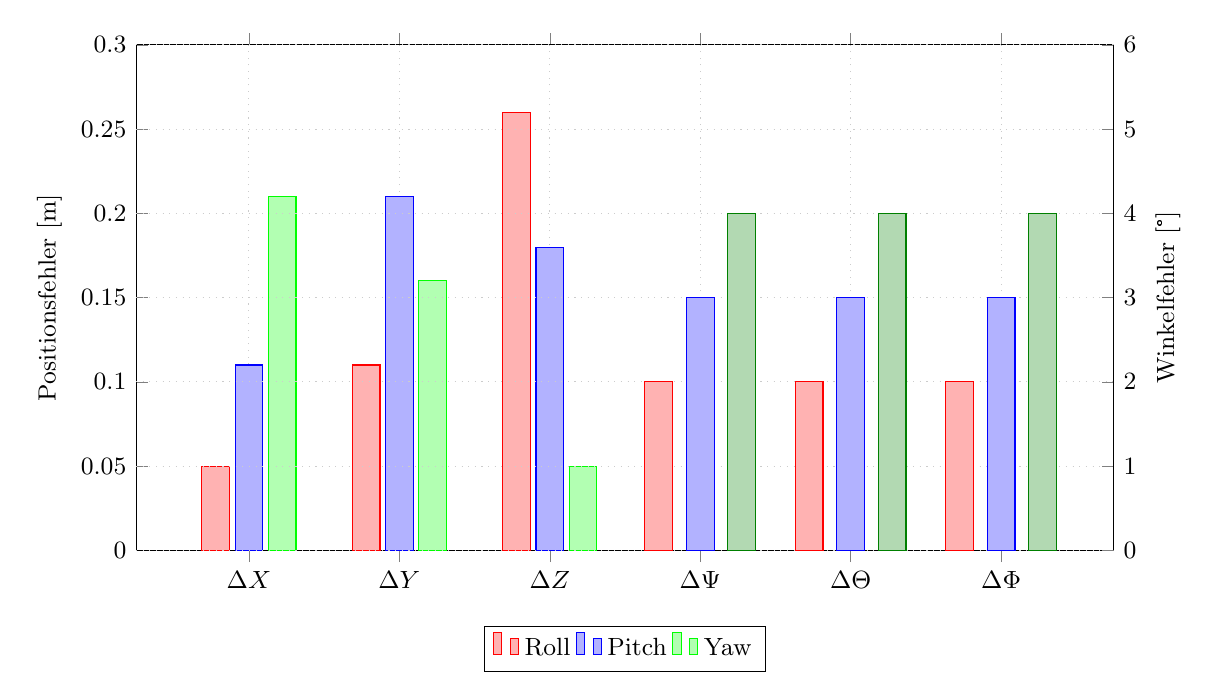
\begin{tikzpicture}
\begin{axis}[
	ybar,
	ymax=0.3,
	ymin=0,
	bar width=10pt,
	scaled y ticks = false,
	y tick label style={/pgf/number format/fixed},
%	enlarge y limits={0.4,upper},
	enlarge x limits=0.15,
	legend style={at={(0.5,-0.15)},
	anchor=north,legend columns=-1},
	ylabel={Positionsfehler \lbrack m\rbrack},
%	symbolic x coords={\Delta,y,z},
	xtick={1,2,3,4,5,6},
	xticklabels={$\Delta X$, $\Delta Y$, $\Delta Z$, $\Delta \Psi$, $\Delta \Theta$, $\Delta \Phi$},
%	xtick=data,
%	every node near coord/.style={/pgf/number format/fixed, anchor=west},
%	nodes near coords,
%	nodes near coords align={vertical},
	width=14cm,
	height=8cm,
	grid=major,
    	grid style={dotted,lightgray!80!white},
    	scaled y ticks = false,
]
\addplot[
%	every node near coord/.append style={xshift=-0.95cm},
%	nodes near coords=\raisebox{0.7cm}{\pgfmathprintnumber\pgfplotspointmeta},
	color=red,
	fill=red!30!white,
	bar shift=-12pt,
] coordinates {(1,0.05) (2,0.11) (3,0.26)};
\addplot[
%	every node near coord/.append style={xshift=-0.41cm},
%	nodes near coords=\raisebox{0.7cm}{\pgfmathprintnumber\pgfplotspointmeta},
	color=blue,
	fill=blue!30!white,
	bar shift=0pt,	
] coordinates {(1,0.11) (2,0.21) (3,0.18)};
\addplot[
%	every node near coord/.append style={xshift=0.12cm},
%	nodes near coords=\raisebox{0.7cm}{\pgfmathprintnumber\pgfplotspointmeta},
	color=green,
	fill=green!30!white,
	bar shift=12pt,	
] coordinates {(1,0.21) (2,0.16) (3,0.05)};
\addplot[fill opacity=0.0,draw=none,] coordinates {(4,0) (5,0) (6,0)};	%dummy
\legend{Roll,Pitch,Yaw}
\end{axis}

\begin{axis}[
%	scale only axis,
	ybar,
	ymax=6,
	ymin=0,
	bar width=10pt,
%	enlarge y limits={0.4,upper},
	enlarge x limits=0.15,
	legend style={at={(0.5,-0.15)},
	anchor=north,legend columns=-1},
	axis y line*=right,
	axis x line=none,
	ylabel={Winkelfehler \lbrack °\rbrack},
%	symbolic x coords={\Delta,y,z},
	xtick={1,2,3,4,5,6},
	xticklabels={$\Delta X$, $\Delta Y$, $\Delta Z$, $\Delta \Psi$, $\Delta \Theta$, $\Delta \Phi$},
%	xtick=data,
%	bar shift=0pt,
%	every node near coord/.style={/pgf/number format/fixed, anchor=west},
%	nodes near coords,
%	nodes near coords align={vertical},
	width=14cm,
	height=8cm,
	grid=major,
    	grid style={dotted,lightgray!80!white},
    	scaled y ticks = false,
]
\addplot[fill opacity=0.0,draw=none,] coordinates {(1,0) (2,0) (3,0)};	%dummy
\addplot[
%	every node near coord/.append style={xshift=-0.9cm},
%	nodes near coords=\raisebox{0.7cm}{\pgfmathprintnumber\pgfplotspointmeta},
	color=Red,
	fill=Red!30!white,
	bar shift=-15pt,	
] coordinates {(4,2) (5,2) (6,2)};
\addplot[
%	every node near coord/.append style={xshift=-0.12cm},
%	nodes near coords=\raisebox{0.7cm}{\pgfmathprintnumber\pgfplotspointmeta},
	color=Blue,
	fill=Blue!30!white,
	bar shift=0pt,	
] coordinates {(4,3) (5,3) (6,3)};
\addplot[
%	every node near coord/.append style={xshift=-0.12cm},
%	nodes near coords=\raisebox{0.7cm}{\pgfmathprintnumber\pgfplotspointmeta},
	color=Green,
	fill=Green!30!white,
	bar shift=15pt,	
] coordinates {(4,4) (5,4) (6,4)};
\end{axis}
\label{fig.loc_loc_rot_fovis}
\end{tikzpicture}
\end{center}

\red[Ergebnisse interpretieren\\]

\subsubsection{Erweitertes Kalman-Filter}
\begin{center}
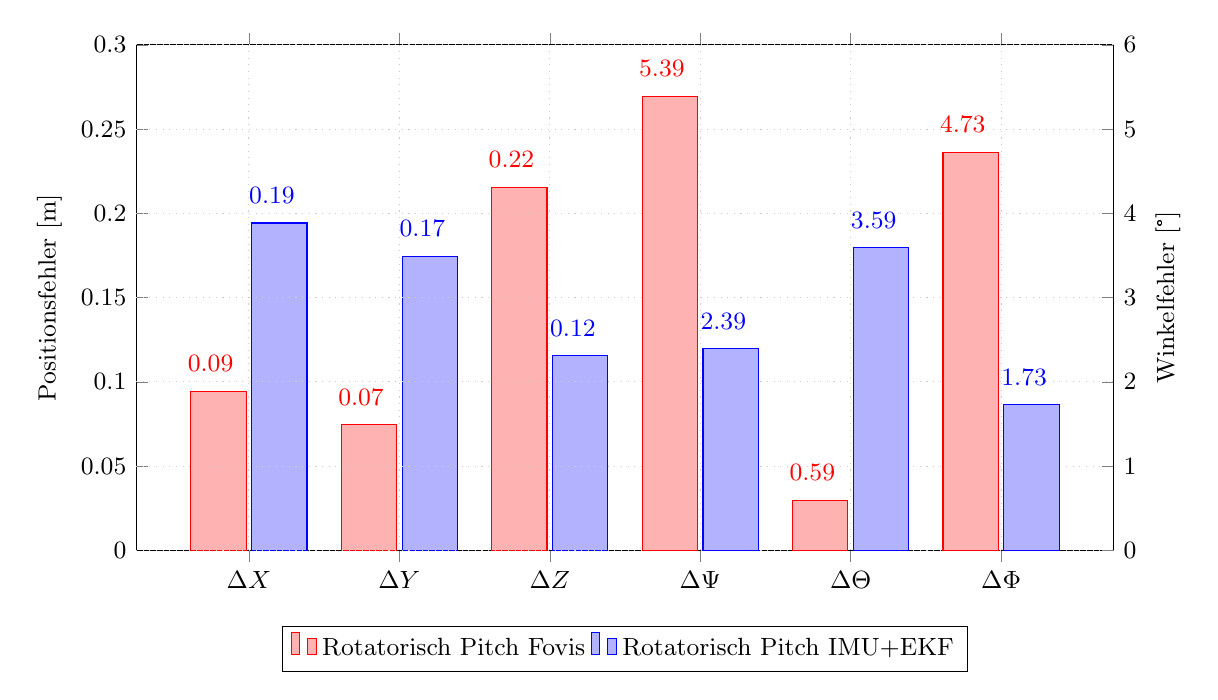
\begin{tikzpicture}
\begin{axis}[
	ybar,
	ymax=0.3,
	ymin=0,
	bar width=20pt,
	scaled y ticks = false,
	y tick label style={/pgf/number format/fixed},
%	enlarge y limits={0.4,upper},
	enlarge x limits=0.15,
	legend style={at={(0.5,-0.15)},
	anchor=north,legend columns=-1},
	ylabel={Positionsfehler \lbrack m\rbrack},
%	symbolic x coords={\Delta,y,z},
	xtick={1,2,3,4,5,6},
	xticklabels={$\Delta X$, $\Delta Y$, $\Delta Z$, $\Delta \Psi$, $\Delta \Theta$, $\Delta \Phi$},
%	xtick=data,
	every node near coord/.style={/pgf/number format/fixed, anchor=west},
	nodes near coords,
	nodes near coords align={vertical},
	width=14cm,
	height=8cm,
	grid=major,
    	grid style={dotted,lightgray!80!white},
    	scaled y ticks = false,
]
\addplot[
	every node near coord/.append style={xshift=-0.9cm},
	nodes near coords=\raisebox{0.7cm}{\pgfmathprintnumber\pgfplotspointmeta},
	color=red,
	fill=red!30!white,
	bar shift=-11pt,
] coordinates {(1,0.0942737252) (2,0.0744944439) (3,0.2154737652)};
\addplot[
	every node near coord/.append style={xshift=-0.12cm},
	nodes near coords=\raisebox{0.7cm}{\pgfmathprintnumber\pgfplotspointmeta},
	color=blue,
	fill=blue!30!white,
	bar shift=11pt,	
] coordinates {(1,0.1942737252) (2,0.1744944439) (3,0.1154737652)};
\addplot[fill opacity=0.0,draw=none,] coordinates {(4,0) (5,0) (6,0)};	%dummy
\legend{Rotatorisch Pitch Fovis,Rotatorisch Pitch IMU+EKF}
\end{axis}

\begin{axis}[
%	scale only axis,
	ybar,
	ymax=6,
	ymin=0,
	bar width=20pt,
%	enlarge y limits={0.4,upper},
	enlarge x limits=0.15,
	legend style={at={(0.5,-0.15)},
	anchor=north,legend columns=-1},
	axis y line*=right,
	axis x line=none,
	ylabel={Winkelfehler \lbrack °\rbrack},
%	symbolic x coords={\Delta,y,z},
	xtick={1,2,3,4,5,6},
	xticklabels={$\Delta X$, $\Delta Y$, $\Delta Z$, $\Delta \Psi$, $\Delta \Theta$, $\Delta \Phi$},
%	xtick=data,
%	bar shift=0pt,
	every node near coord/.style={/pgf/number format/fixed, anchor=west},
	nodes near coords,
	nodes near coords align={vertical},
	width=14cm,
	height=8cm,
	grid=major,
    	grid style={dotted,lightgray!80!white},
    	scaled y ticks = false,
]
\addplot[fill opacity=0.0,draw=none,] coordinates {(1,0) (2,0) (3,0)};	%dummy
\addplot[
	every node near coord/.append style={xshift=-0.9cm},
	nodes near coords=\raisebox{0.7cm}{\pgfmathprintnumber\pgfplotspointmeta},
	color=Red,
	fill=Red!30!white,
	bar shift=-11pt,	
] coordinates {(4,5.3910094725) (5,0.5944624236) (6,4.7266768476)};
\addplot[
	every node near coord/.append style={xshift=-0.12cm},
	nodes near coords=\raisebox{0.7cm}{\pgfmathprintnumber\pgfplotspointmeta},
	color=Blue,
	fill=Blue!30!white,
	bar shift=11pt,	
] coordinates {(4,2.3910094725) (5,3.5944624236) (6,1.7266768476)};
\end{axis}
\label{fig.loc_loc_rot_ekf_roll}
\end{tikzpicture}
\end{center}

\begin{center}
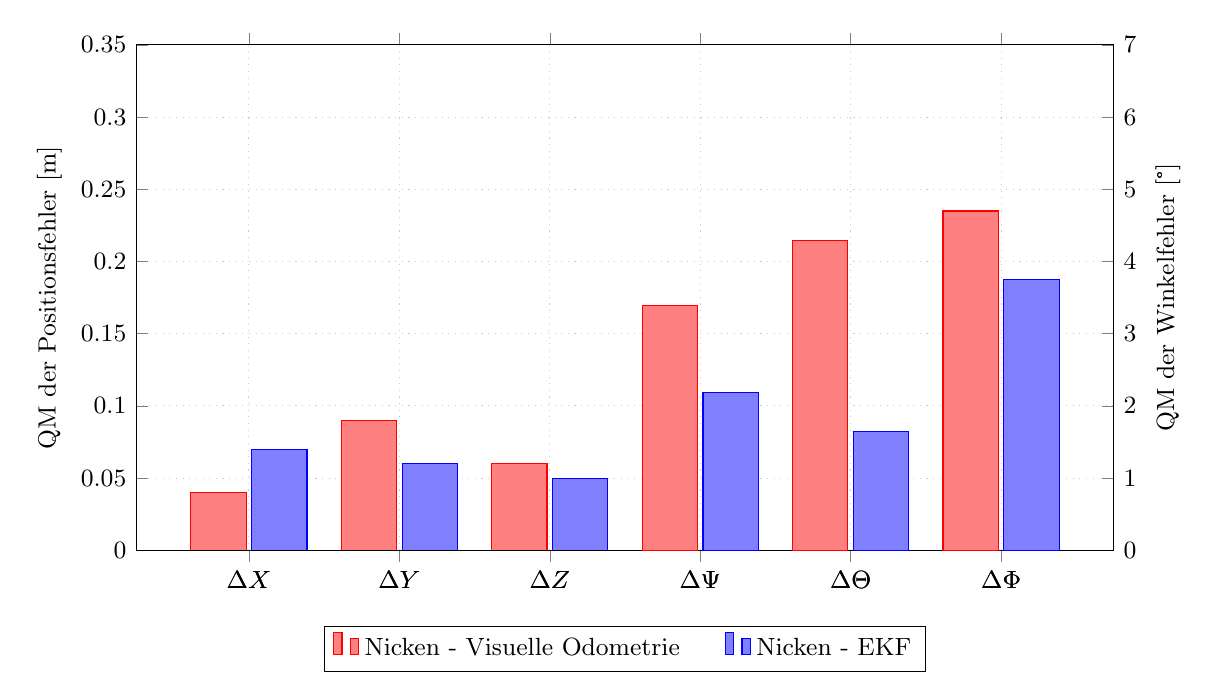
\begin{tikzpicture}
\begin{axis}[
	ybar,
	ymax=0.35,
	ymin=0,
	bar width=20pt,
	scaled y ticks = false,
	y tick label style={/pgf/number format/fixed},
%	enlarge y limits={0.4,upper},
	enlarge x limits=0.15,
	legend style={at={(0.5,-0.15)},
	legend style={/tikz/every even column/.append style={column sep=0.5cm}},
	anchor=north,legend columns=-1},
	ylabel={QM der Positionsfehler \lbrack m\rbrack},
%	symbolic x coords={\Delta,y,z},
	xtick={1,2,3,4,5,6},
	xticklabels={$\Delta X$, $\Delta Y$, $\Delta Z$, $\Delta \Psi$, $\Delta \Theta$, $\Delta \Phi$},
%	xtick=data,
%	every node near coord/.style={/pgf/number format/fixed,/pgf/number format/use comma, anchor=west},
%	nodes near coords,
%	nodes near coords align={vertical},
	width=14cm,
	height=8cm,
	grid=major,
    	grid style={dotted,lightgray!80!white},
    	scaled y ticks = false,
]
\addplot[
%	every node near coord/.append style={xshift=-0.9cm},
%	nodes near coords=\raisebox{0.7cm}{\pgfmathprintnumber\pgfplotspointmeta},
	color=red,
	fill=red!50!white,
	bar shift=-11pt,
] coordinates {(1,0.04) (2,0.09) (3,0.06)};
\addplot[
%	every node near coord/.append style={xshift=-0.12cm},
%	nodes near coords=\raisebox{0.7cm}{\pgfmathprintnumber\pgfplotspointmeta},
	color=blue,
	fill=blue!50!white,
	bar shift=11pt,	
] coordinates {(1,0.07) (2,0.06) (3,0.05)};
\addplot[fill opacity=0.0,draw=none,] coordinates {(4,0) (5,0) (6,0)};	%dummy
\legend{Nicken - Visuelle Odometrie,Nicken - EKF}
\end{axis}

\begin{axis}[
%	scale only axis,
	ybar,
	ymax=7,
	ymin=0,
	bar width=20pt,
%	enlarge y limits={0.4,upper},
	enlarge x limits=0.15,
	legend style={at={(0.5,-0.15)},
	anchor=north,legend columns=-1},
	axis y line*=right,
	ylabel={QM der Winkelfehler \lbrack °\rbrack},
%	symbolic x coords={\Delta,y,z},
	xtick={1,2,3,4,5,6},
	xticklabels={$\Delta X$, $\Delta Y$, $\Delta Z$, $\Delta \Psi$, $\Delta \Theta$, $\Delta \Phi$},
%	xtick=data,
%	bar shift=0pt,
%	every node near coord/.style={/pgf/number format/fixed,/pgf/number format/use comma, anchor=west},
%	nodes near coords,
%	nodes near coords align={vertical},
	width=14cm,
	height=8cm,
    	scaled y ticks = false,
]
\addplot[fill opacity=0.0,draw=none,] coordinates {(1,0) (2,0) (3,0)};	%dummy
\addplot[
%	every node near coord/.append style={xshift=-0.9cm},
%	nodes near coords=\raisebox{0.7cm}{\pgfmathprintnumber\pgfplotspointmeta},
	color=red,
	fill=red!50!white,
	bar shift=-11pt,	
] coordinates {(4,3.39) (5,4.29) (6,4.70)};
\addplot[
%	every node near coord/.append style={xshift=-0.12cm},
%	nodes near coords=\raisebox{0.7cm}{\pgfmathprintnumber\pgfplotspointmeta},
	color=blue,
	fill=blue!50!white,
	bar shift=11pt,	
] coordinates {(4,2.18) (5,1.64) (6,3.75)};
\end{axis}
\end{tikzpicture}
\end{center}

\red[Ergebnisse interpretieren\\]

%\subsection{Rotation Roll IMU+KALMAN}

\section{Projektionsgenauigkeit}
Die Genauigkeit der Projektion virtueller Modelldaten wird unter Verwendung einer externen Kamera durchgeführt. Diese wird zunächst analog zum Vorgehen für die RGB-Kamera des Kinect Sensors kalibriert (siehe \kapitel{chap.calib}), wodurch eine objektive Betrachtung der Projektionsgenauigkeit ermöglicht wird. Für die Untersuchung wird ein Markerfeld auf einer ebenen Unterlage fixiert und im Sicht- und Projektionsfeld des \kps{s} platziert. Das Markerfeld wird mittels der RGB-Kamera erfasst um die Transformation des \kps{s} relativ zum Markerfeld zu bestimmen.\\

Die bekannte Transformation zwischen Kamera- und Projektorkoordinaten ermöglicht daraufhin die Zuordnung der detektierten 3D-Koordinaten des Markerfeldes zu den 2D-Koordinaten des Projektorbildes. Um die Projektionsgenauigkeit zu überprüfen wird mittels des Projektors ein weiteres Markerfeld projiziert, welches bezogen auf die Projektorkoordinaten deckungsgleich mit dem realen Markerfeld ist. \red[\abb{fig.arprojected}]\\
\red[Umweg über Modellumgebung beschreiben?\\]

\begin{figure}[!ht]
	\begin{center}
		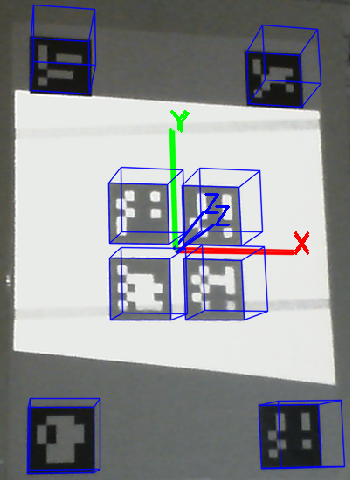
\includegraphics[scale=0.5]{board_eval_cropped}
		\caption{AR Marker real und projiziert}
		\label{fig.arprojected}
	\end{center}
	%\vspace*{-8mm}
\end{figure}

Die externe Kamera wird nun eingesetzt, um beide Markerfelder gleichzeitig zu erfassen und die Abweichungen zwischen den Feldern bezüglich Position und Orientierung zu bestimmen. Dabei werden die Positionierungen sowohl des \kps{s} als auch der externen Kamera während der Untersuchungen variiert. Der gesamte Aufbau der durchgeführten Untersuchung ist in \abb{fig.projsetup} dargestellt.

\begin{figure}[ht]
	\begin{center}%
		\includesvgnew[1]{images/projection_validation_cropped}%
		\caption{Aufbau zur Überprüfung der Projektionsgenauigkeit}
		\label{fig.projsetup}
	\end{center}
	%\vspace*{-8mm}
\end{figure}

\red[Die Ergebnisse der $n=6$ Messreihen sind als Box-Whisker-Plot in \abb{fig.boxplot_proj} dargestellt.]

\begin{figure}[!ht]
\begin{center}
\begin{tikzpicture}[trim axis left, trim axis right]
  \begin{axis}[
    	ytick={-30,-20,...,30},
    		minor y tick num=1,
    		ymax=35,
    		ymin=-35,
    		ylabel=Positionsfehler \lbrack mm\rbrack,
    		xtick={1,2,...,6},
    		x tick label style={align=center},
    		xticklabels={$\Delta X$, $\Delta Y$, $\Delta Z$, $\Delta \Psi$, $\Delta \Theta$, $\Delta \Phi$},
    		boxplot/draw direction=y,
    		width=14cm,
    		height=8cm,
    		grid=major,
    		grid style={dotted,lightgray!80!white},
    ]
    \addplot+[color=red,mark=x,
    		boxplot prepared={
      		lower whisker=-7.2937458753,
      		lower quartile=-2.2697057575,
      		median=-0.5078930408,
      		upper quartile=2.5787912309,
      		upper whisker=5.2836090326,
      		box extend=0.5,
      		draw position=1,
    		},
    ] coordinates {};
    %table[row sep=\\,y index=0] {0.0\\}; %Ausreisser
    \addplot+[color=Green,mark=x,
    		boxplot prepared={
      		lower whisker=-5.6481547653,
      		lower quartile=0.8273310959,
      		median=2.7935747058,
      		upper quartile=6.1452584341,
      		upper whisker=6.959207356,
			box extend=0.5,
			draw position=2,
		},
    ] coordinates {};
    %table[row sep=\\,y index=0] {0.0\\}; %Ausreisser
    \addplot+[color=blue,mark=x,
    		boxplot prepared={
      		lower whisker=-30.851304531,
      		lower quartile=-12.757569552,
      		median=5.149245262,
      		upper quartile=11.0025405888,
      		upper whisker=22.670924664,
			box extend=0.5,
			draw position=3,
		},
    ] coordinates {};
    \addplot+[color=blue,mark=x,
    		boxplot prepared={
      		lower whisker=-30.851304531,
      		lower quartile=-12.757569552,
      		median=5.149245262,
      		upper quartile=11.0025405888,
      		upper whisker=22.670924664,
			box extend=0.5,
			draw position=6,
			every box/.style={draw=none},
			every whisker/.style={draw=none},
			every median/.style={draw=none},
		},
    ] coordinates {};
    \addplot[fill opacity=0.0,draw=none,] coordinates {(4,0) (5,0) (6,0)};	%dummy
    %table[row sep=\\,y index=0] {0.0\\}; %Ausreisser
  \end{axis}
  
  \begin{axis}[
    	ytick={-15,-10,...,15},
    		minor y tick num=1,
    		ymax=17.5,
    		ymin=-17.5,
    		ylabel=Winkelfehler \lbrack °\rbrack,
    		xtick={1,2,...,6},
    		x tick label style={align=center},
    		xticklabels={$\Delta X$, $\Delta Y$, $\Delta Z$, $\Delta \Psi$, $\Delta \Theta$, $\Delta \Phi$},
    		boxplot/draw direction=y,
    		width=14cm,
    		height=8cm,
		axis y line*=right,
%		axis x line=none,
    		grid=major,
    		grid style={dotted,lightgray!80!white},
    ]
    %\addplot[fill opacity=0.0,draw=none,] coordinates {(1,0) (2,0) (3,0)};	%dummy
    \addplot+[color=red,mark=x,
    		boxplot prepared={
      		lower whisker=-16.4794351302,
      		lower quartile=-9.598333392,
      		median=3.2716409046,
      		upper quartile=9.967066701,
      		upper whisker=10.9694603209,
      		box extend=0.5,
      		draw position=4,
    		},
    ] coordinates {};
    %table[row sep=\\,y index=0] {0.0\\}; %Ausreisser
    \addplot+[color=Green,mark=x,
    		boxplot prepared={
      		lower whisker=-15.2919184736,
      		lower quartile=-8.5080543959,
      		median=-3.0498185813,
      		upper quartile=2.0169290245,
      		upper whisker=5.2929529487,
			box extend=0.5,
			draw position=5,
		},
    ] coordinates {};
        \addplot+[color=blue,mark=x,
    		boxplot prepared={
      		lower whisker=-0.7043281462,
      		lower quartile=-0.1649735629,
      		median=0.1678607749,
      		upper quartile=0.4320938776,
      		upper whisker=2.0949206723,
			box extend=0.5,
			draw position=6,
		},
    ] coordinates {};
    %table[row sep=\\,y index=0] {0.0\\}; %Ausreisser
    \addplot+[color=blue,mark=x,
    		boxplot prepared={
      		lower whisker=-30.851304531,
      		lower quartile=-12.757569552,
      		median=5.149245262,
      		upper quartile=11.0025405888,
      		upper whisker=22.670924664,
			box extend=0.5,
			draw position=1,
			every box/.style={draw=none},
			every whisker/.style={draw=none},
			every median/.style={draw=none},
		},
    ] coordinates {};
    \addplot[fill opacity=0.0,draw=none,] coordinates {(1,1) (2,2) (3,1)};	%dummy
    %table[row sep=\\,y index=0] {0.0\\}; %Ausreisser
  \end{axis}
\end{tikzpicture}
\caption{Box-Whisker-Plot der Differenzen zwischen realem und projiziertem Markerfeld}
\label{fig.boxplot_proj}
\end{center}
\vspace{-5mm}
\end{figure}

%\begin{figure}
%\begin{center}
%\begin{tikzpicture}[trim axis left, trim axis right]
%  \begin{axis}[
%    	ytick={-30,-20,...,30},
%    		minor y tick num=3,
%    		ymax=35,
%    		ymin=-35,
%    		ylabel=Y-Achse \lbrack mm\rbrack,
%    		xtick={1,...,3},
%    		x tick label style={align=center},
%    		xticklabels={$\Delta X$,$\Delta Y$,$\Delta Z$},
%    		boxplot/draw direction=y,
%    		width=14cm,
%    		height=8cm,
%    		grid=major,
%    		grid style={dotted,lightgray!80!white},
%    ]
%    \addplot+[color=red,mark=x,
%    		boxplot prepared={
%      		lower whisker=-7.2937458753,
%      		lower quartile=-2.2697057575,
%      		median=-0.5078930408,
%      		upper quartile=2.5787912309,
%      		upper whisker=5.2836090326,
%      		box extend=0.5,
%    		},
%    ] coordinates {};
%    %table[row sep=\\,y index=0] {0.0\\}; %Ausreisser
%    \addplot+[color=Green,mark=x,
%    		boxplot prepared={
%      		lower whisker=-5.6481547653,
%      		lower quartile=0.8273310959,
%      		median=2.7935747058,
%      		upper quartile=6.1452584341,
%      		upper whisker=6.959207356,
%			box extend=0.5,
%		},
%    ] coordinates {};
%    %table[row sep=\\,y index=0] {0.0\\}; %Ausreisser
%    \addplot+[color=blue,mark=x,
%    		boxplot prepared={
%      		lower whisker=-30.851304531,
%      		lower quartile=-12.757569552,
%      		median=5.149245262,
%      		upper quartile=11.0025405888,
%      		upper whisker=22.670924664,
%%      		lower whisker=-9.7615455743,
%%      		lower quartile=-4.0365747411,
%%      		median=1.6292533837,
%%      		upper quartile=3.4812726082,
%%      		upper whisker=7.173222257,
%			box extend=0.5,
%		},
%    ] coordinates {};
%    %table[row sep=\\,y index=0] {0.0\\}; %Ausreisser
%  \end{axis}
%\end{tikzpicture}
%\caption{Box-Whisker-Plot}
%\label{fig.boxplot_proj}
%\end{center}
%\vspace{-3mm}
%\end{figure}

\red[Öffnungswinkel $\sim$ 30°, dadurch Faktor 16/9 für Fehlerwerte in z-Richtung. Sogar (16/9)²!! für Detektion+Projektion? Dann würden sich die Werte auf jeden Fall stark annähern\\Bereinigtes Diagramm zeigen? welchen Nutzen?\\]

\red[Nennen, dass Boxplot ganze Messreihe abbildet! Oder umwandeln zu 5/95 Perzentil?\\]

%\section{Benutzerinteraktion}

%\begin{figure}[!ht]
\vspace{3mm}
\begin{center}
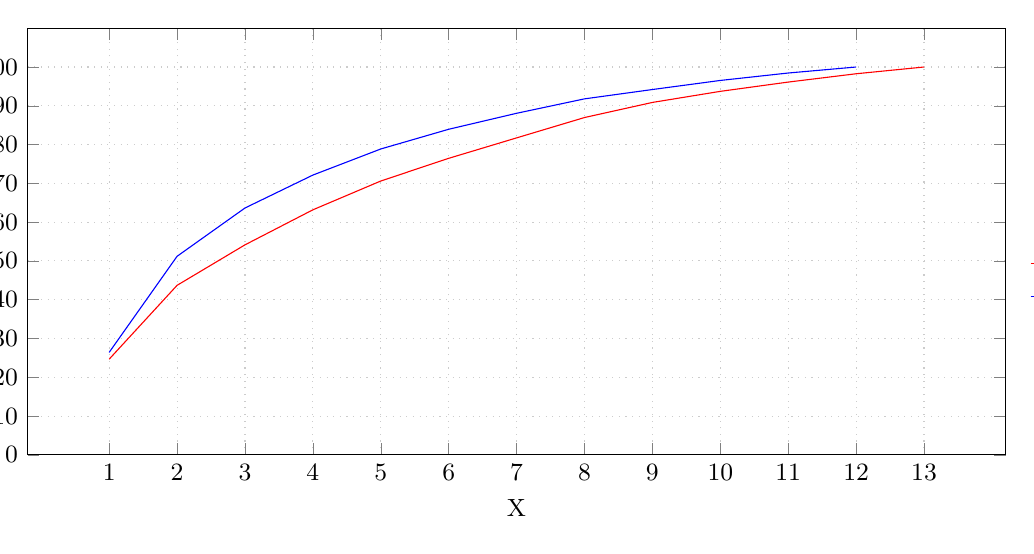
\begin{tikzpicture}[trim axis left, trim axis right]
	\begin{axis}[
		xlabel=X,
		ylabel=Y,
		xtick={1,...,13},
		ymin=0,
		ytick={0,10,...,100},
		legend style={
			at={(1,0.5)},
			xshift=0.2cm,
			anchor=north west,
			nodes=right,
			draw=none
		},
		grid=major,
   		grid style={dotted,lightgray!80!white},
		%axis lines=left
		width=14cm,
		height=7cm,
	]
	\addplot[color=red] coordinates{
		(1,24.6718)
		(2,43.7092)
		(3,54.14785132)
		(4,63.1821339)
		(5,70.60866985)
		(6,76.45681086)
		(7,81.7263871)
		(8,86.97406846)
		(9,90.86684525)
		(10,93.72329021)
		(11,96.11621437)
		(12,98.25885879)
		(13,100)		
	};
	\addplot[color=blue] coordinates{
		(1,26.42529337)
		(2,51.19458535)
		(3,63.64859236)
		(4,72.13773673)
		(5,78.8676646)
		(6,83.94694845)
		(7,88.06842906)
		(8,91.7882484)
		(9,94.19470806)
		(10,96.53607266)
		(11,98.45170481)
		(12,100)
		
	};
	\legend{Testa,Testb}
	\end{axis}
\end{tikzpicture}
\end{center}
\vspace{-3mm}
\caption{test1}
\label{fig.test1}
\vspace{3mm}
\end{figure}

\begin{figure}[ht]
\centering
\begin{tikzpicture}
\begin{axis}[
xlabel={Zeit},
ylabel={Position},
ymin=0,
ymax=6,
width=100mm,
height=80mm,
ytick={0,1,...,5},
legend style={at={(1,1)},	anchor=north east, xshift=-1mm,	yshift=-1mm}
]
\pgfplotstableread{plot/test.txt}\datatable
\addplot[color=red,mark=square*] table[x index=0,y index=1] from \datatable;
%\addplot[no markers] table[x index=0,y index=3] from \datatable;
%\addplot[no markers] table[y = Leistung] {plot/test.txt}  ;
\legend{test}
\end{axis}
\end{tikzpicture}
\caption{test2}
\label{fig.test2}
\end{figure}

\begin{figure}
\begin{center}
\begin{tikzpicture}[trim axis left, trim axis right]
  \begin{axis}[
    	ytick={0,0.1,...,1.1},
    		minor y tick num=5,
    		ymax=1.1,
    		ylabel=Y-Achse,
    		xtick={1,...,4},
    		x tick label style={align=center},
    		xticklabels={A, B},
    		boxplot/draw direction=y,
    		width=8cm,
    		height=8cm,
    		thick,
    ]
%    \addplot+[color=red,mark=x,
%    		boxplot prepared={
%      		lower whisker=,
%      		lower quartile=,
%      		median=,
%      		upper quartile=,
%      		upper whisker=
%    		},
%    ] %coordinates {};
%    table[row sep=\\,y index=0] {0.7054\\ 0.9773\\  0.9763\\ 0.9698\\ 0.7118\\ 0.6919\\ 0.9727\\ 0.7006\\ 0.974\\ 0.7077\\}; %Ausreisser
    \addplot+[color=Green,mark=x,
    		boxplot prepared={
      		median=0.3036,
      		upper quartile=0.34925,
      		lower quartile=0.2674,
      		upper whisker=0.5597,
      		lower whisker=0.18718
		},
    ] %coordinates {};
    table[row sep=\\,y index=0] {0.6045\\ 0.1818\\ 0.5826\\ 0.5688\\ 0.1814\\ 0.1825\\ 0.5750\\ 0.1783\\ 0.6312\\ 0.1793\\}; %Ausreisser
  \end{axis}
\end{tikzpicture}
\caption{Box-Whisker-Plot}
\label{fig.error_boxplot}
\end{center}
\vspace{-3mm}
\end{figure}
